\chapter{Ciclo 1: Geração de novas sequências com LSTM}
\label{chap:lstm}

No primeiro ciclo de estudos, exploramos a implementação de um modelo preditivo gerador de novas sequências baseado em entradas anteriores. Utilizamos como método principal a rede neural LSTM (\textit{Long Short-Term Memory}) para implementá-lo.

Neste Capítulo, descreveremos a metodologia utilizada para realizar os experimentos, demonstraremos seus resultados e, a partir deles, tiraremos conclusões, de acordo com as métricas de sucesso descritas na \secref{sec:success_metrics}.

\section{Metodologia dos experimentos}
\label{sec:lstm-metodology}

Para definir nossa metodologia, precisamos estabelecer seguintes passos necessários para realizar nossos experimentos: (1) como as camadas da rede neural foram organizadas; (2) a formatação dos dados de entrada para aprendizagem; (3) o processo de previsão das sequências.

\subsection{Camadas da rede neural}

A API Keras \cite{keras}, uma biblioteca em Python voltada para desenvolvimento de aplicações \textit{deep learning}, implementa a camada \textit{LSTM} em seu modelo \textit{Sequential}. Em nossos experimentos, utilizaremos uma camada de \textit{input}, uma camada LSTM, que realizará as previsões, e uma camada \textit{Dense}, que reunirá as camadas em uma única lista de \textit{output}. A \figref{fig:lstm-rnn} ilustra essa rede neural, considerando que queremos prever sequências simulando uma latência de 50 ms.

\begin{figure}[htbp]
    \centering
    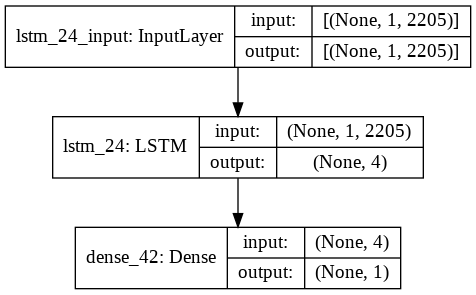
\includegraphics[width=0.5\textwidth]{images/lstm-rnn.png}
    \caption{Visualização da rede neural utilizada nos experimentos com LSTM para uma latência simulada de 50 ms.}
    \label{fig:lstm-rnn}
\end{figure}

\subsection{Formatação dos dados de aprendizagem}
\label{subsec:input_lstm}

O nosso conjunto de dados, como exemplificado na \secref{sec:data_gathering}, consistirá de músicas com apenas um instrumento isolado, de forma a simular a transmissão do músico remoto. A música é representada como uma lista de sinais digitais, com uma frequência de 44.100 valores a cada segundo (44.1 KHz). Com um \textit{bit depth} de 16 bits, os valores estão contidos no intervalo $[-32.768, +32.767]$.

Como entrada para realizar a aprendizagem, o modelo \textit{Sequential} requer duas listas:

\begin{enumerate}
    \item Uma lista $X$ de sequências numéricas de tamanho $LB$ e;
    \item Uma lista $Y$ de sequências numéricas futuras de tamanho $LB$.
\end{enumerate}

As listas estão organizadas de forma que, dado a lista $X_i$, a lista $Y_i$ representa o que veio em seguida - isto é, para uma sequência na posição $i$ na lista $X$, a sequência na mesma posição $i$ na lista $Y$ representa a sequência que veio logo a seguir. O valor de $LB$, representando o \textit{lookback} que devemos utilizar para analisar a lista do passado e a geração de previsões, serve como o número de elementos de cada lista $X_i$ e $Y_i$.

Por exemplo, supondo que queremos analisar a sequência numérica $(1, 2, 3, 4, 5, 6)$. Para um $LB = 2$, as listas de entrada serão organizadas de tal forma:

\begin{equation}
\begin{split}
    X = ((1, 2), (3, 4)) \\
    Y = ((3, 4), (5, 6))
\end{split}
\end{equation}

Note que o conjunto $X$ não possui a sequência $(5,6)$. Isso se dá pois, dado o valor de $LB = 2$, não há nenhuma outra sequência futura de tamanho $2$.

Para simplificar o processamento da aprendizagem e da previsão, normalizamos as sequências numéricas no intervalo $[-1, +1]$.

Em nossos experimentos, utilizamos os dois primeiros segundos da introdução da música \textit{Hotel California} (\textit{Eagles}, 1976), com a trilha isolada do violão acústico. Tal sessão se repete em um total de três vezes ao longo da música, porém, com diferentes execuções. A primeira delas, então, é usada como treinamento.

O valor do \textit{lookback}, em nossa adaptação, representa o tamanho da janela de previsão. A escolha desse valor está intrinsecamente conectada ao sucesso do algoritmo - valores pequenos possuem pouca informação, porém, são mais rápidos para processar; reciprocamente, o inverso ocorre com valores maiores. É importante mencionar que esse valor necessita ser maior que a latência apresentada pelo transporte dos pacotes pela Internet, afinal, queremos compensá por ela ao realizar previsões.

Portanto, para calcular o valor de $LB$, precisamos definir o valor de $LAG$, que simula a latência apresentada pela Internet. Em nossos experimentos, escolhemos dois valores: (1) 50 ms e (2) 100 ms. O primeiro valor foi definido utilizando de uma média de testes de \textit{ping} entre Recife e o servidor 8.8.8.8, hospedado pelo Google e localizado no estado da Califórnia, Estados Unidos. O segundo é o dobro desse valor, de forma a compensar por possíveis picos de latência apresentados pela incerteza da entrega de pacotes pela Internet.

Então, dado os valores $SR$ e $LAG$, onde $SR$ representa o \textit{sample rate} das sequências de áudio medido em KHz (\textit{valores} por segundo) e $LAG$ a latência simulada da Internet medida em (milissegundos), podemos calcular $LB$ aplicando a seguinte fórmula:

\begin{equation}
    LB = \frac{SR}{1.000} * LAG
\end{equation}

A divisão entre $SR$ e 1.000 nos dá a quantidade de \textit{samples} a cada milissegundo de áudio. Finalmente, a multiplicação desse valor por $LAG$ nos dá a quantidade de \textit{samples} por cada unidade de latência apresentada pela Internet. Esse cálculo, portanto, nos dá o total de valores que o modelo precisará prevê para compensar pelo tempo de transporte dos pacotes. Portanto, para o valor de latência de 50 ms, $LB = 2.205$ e; para 100 ms, $LB = 4.410$.

Para o treinamento do modelo \textit{Sequential}, precisamos definir, também, um valor $E$ de iterações rodadas no treinamento, denominadas \textit{epochs}. Definimos $E = 3$, pois, em nossos experimentos, percebemos que a função de perda calculada pelo modelo não apresentava mudanças significativas depois de três iterações.

Apesar de não ser uma das métricas de sucesso definidas na \secref{sec:success_metrics}, o tempo de treinamento também foi registrado em nossos experimentos.

Definidos os valores de $X$, $Y$, $LB$ e $E$, podemos, então treinar nossa rede neural. Uma vez treinado, podemos usá-la para realizar as predições.

\subsection{Processo de previsão}

Nos experimentos de nossas predições, precisamos organizar nossos dados de teste. Escolhemos a terceira repetição da introdução tocada em \textit{Hotel California} pois, em análise manual, soaram semelhantes entre si, porém, com algumas pequenas improvisações. Por exemplo, em algumas transições entre acordes, é tocado uma nota intermediária, o que não foi observado na primeira repetição da introdução. Essa característica é ideal para uma simulação de um ambiente musical \textit{online} colaborativo - a mesma sequência de acordes foi tocada, porém, com leves variações da forma que é performada.

Uma vez treinado, o modelo requer uma lista $Z$, no mesmo formato que a lista $X$, definida na \subsecref{subsec:input_lstm} - uma conjunto de subconjuntos de tamanho $LB$. Além disso, precisaremos realizar a normalização inversa da previsão para retornar os valores ao intervalo original de $[-32.768, +32.767]$ para, de fato, podermos representar as previsões em arquivos WAV.

Portanto, para rodar as previsões com o arquivo completo da introdução de \textit{Hotel California}, precisamos dividir tal arquivo durações de $LAG$ ms e, para cada uma, convertê-las no formato requerido da lista $Z$.

Como uma das métricas de sucesso, definidas na \secref{sec:success_metrics}, é o tempo necessário para gerar as previsões, medimos o tempo para formatar cada arquivo de duração $LAG$ ms e o de geração das previsões, para cada lista $Z$.

Ao final de todas as previsões, convertemos todas as sequências de sinais digitais para um arquivo WAV para análise manual dos áudios produzidos \footnote{O áudio gerado pode ser encontrado em \url{https://cutt.ly/cvNkBna}.}.
\section{Avaliação}

Para analisar a efetividade desse modelo, vamos analisar sob a ótica os critérios de avaliação, definidos na \secref{sec:success_metrics}.

\subsection{Corretude das previsões}

Para cada um dos valores de $LAG$, definidos na \secref{sec:lstm-metodology}, todas as previsões realizadas tenderam a "repetir" as sequências de áudio de entrada. Comparando os sinais digitais do arquivo de teste e os gerados na previsão, ilustrados na \figref{fig:lstm-repetition-results}, é possível notar que, quando alinhado com a sequência real de teste, não há nenhuma correspondência. No entanto, ao compararmos com os dados de entrada, isto é, o que construímos a lista $Z$, é possível notar uma clara semelhança. O formato da onda sonora foi mantido, diferindo apenas por sua amplitude.

Ademais, os áudios previstos soaram distorcidos, consequência das diferenças de amplitude encontradas nos sinais digitais da previsão contra a sequência de entrada.

Esses resultados foram observados em todas as janelas de entrada, tanto para os valores de $LAG$ 50 ms e 100 ms.

\begin{figure}
     \centering
     \begin{subfigure}[b]{0.49\textwidth}
         \centering
         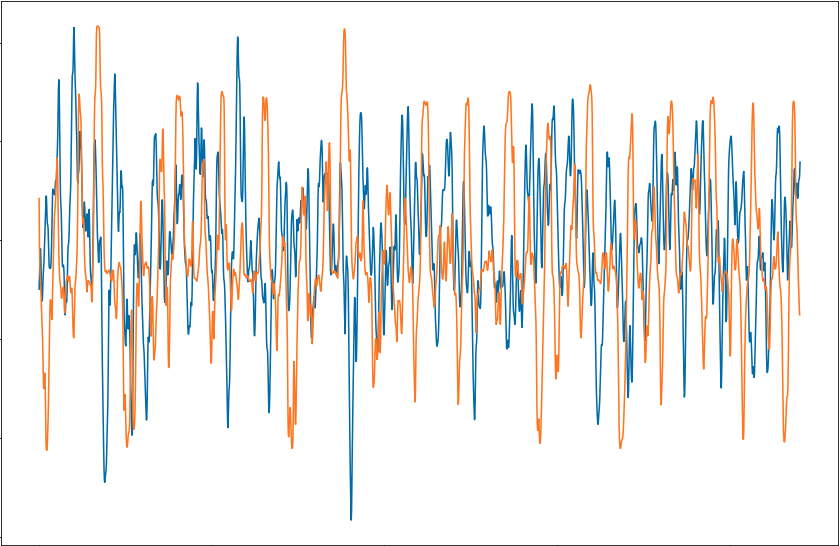
\includegraphics[width=\textwidth]{images/lstm-after.png}
         \caption{Previsão alinhada com a sequência real de teste.}
         \label{fig:y equals x}
     \end{subfigure}
     \hfill
     \begin{subfigure}[b]{0.49\textwidth}
         \centering
         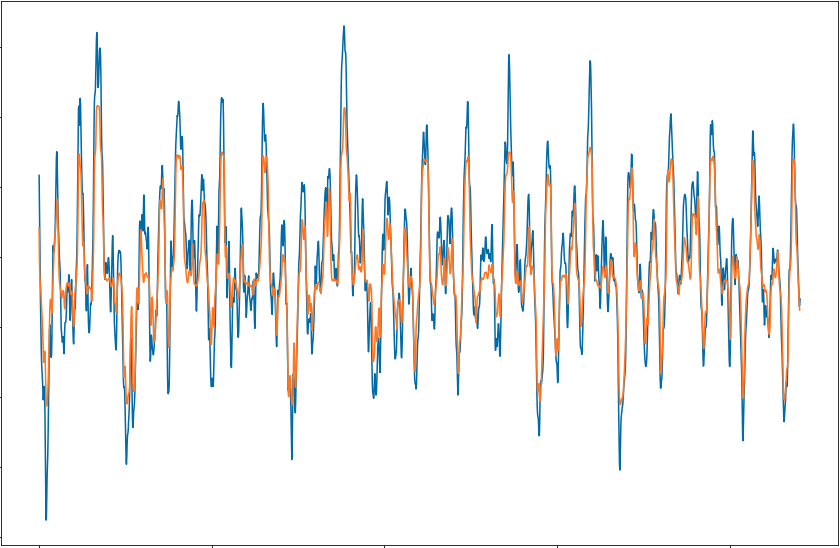
\includegraphics[width=\textwidth]{images/lstm-before.png}
         \caption{Previsão alinhada com a sequência de entrada.}
         \label{fig:three sin x}
     \end{subfigure}
        \caption{Comparação entre as sequências digitais geradas na previsão de uma das listas $Z$, em laranja, com (a) a sequência real de teste e (b) a sequência de entrada, ambas em azul, para o valor $LAG = 50 ms$.}
        \label{fig:lstm-repetition-results}
\end{figure}

Caso aplicássemos esse modelo em uma aplicação real, efetivamente estaríamos repetindo os dados transmitidos e, como discutido no \chapref{chap:solution_propositon}, retornaremos ao problema que as soluções \textit{delay-based} enfrentam. Portanto, não podemos atestar a corretude das previsões para o modelo preditivo gerador de novas sequências.

\subsection{Tempo de geração de previsões}

Na \tabref{tab:lstm-time-results}, podemos observar as médias de tempo para gerar as previsões para cada valor de $LAG$ testado, assim com o tempo médio de treinamento. É notável que, para nenhum dos dois valores, o tempo de previsão foi menor que o tempo da janela de previsão. Dessa forma, podemos afirmar que este modelo preditivo, como foi implementado, não satisfaz a métrica de sucesso para o tempo de previsão.

Ademais, vale notar que, apesar de não ser uma métrica de sucesso, que o tempo médio de treinamento foi relativamente alto, além de depender do valor de $LAG$.

\begin{table}[ht!]
    \centering
    \begin{tabular}{|c||c|c|}
        \hline
        
        Valor de LAG & Média de tempo de previsão & Média de tempo de treinamento por epoch \\
        
        \hline
        \hline
        
        50 ms & 150 ms & 55 s  \\ 
        \hline
        
        100 ms & 380 ms & 127 s \\ 
        \hline
    \end{tabular}
    \caption{Tabela comparando os tempos médios para gerar as previsões e para treinar os modelos para os valores 50 ms e 100 ms de simulação de latência da Internet.}
    \label{tab:lstm-time-results}
\end{table}
